\documentclass{beamer}
\setbeamercovered{transparent}

\usepackage{epstopdf}
\usepackage[inline]{asymptote}

\mode<presentation> %?

\usetheme{Frankfurt}
\usepackage{helvet}
\usepackage{mathptmx}
%\usefonttheme{professionalfonts}
\usefonttheme[onlymath]{serif}
\usefonttheme{structurebold}

%\renewcommand{\familydefault}{Futura}
%\setsansfont{Verdana}

\setlength{\unitlength}{\paperwidth}

% width, height, title, content
\newcommand{\SizedBlock}[4]{
  \begin{block}{#3}
    \parbox[t][#2\paperwidth][t]{#1\paperwidth}{#4}    
  \end{block}
}

% w1, c1, w2, c2
\newcommand{\TwoColumns}[4]{
  \vspace{-0.02\paperwidth}
  \begin{columns}[t]
    \begin{column}{#1\paperwidth}
      #2
    \end{column}\hspace{-0.02\paperwidth}
    \begin{column}{#3\paperwidth}
      #4
    \end{column}
  \end{columns}
}

% w1, c1, w2, c2, w3, c3
\newcommand{\ThreeColumns}[6]{
  \vspace{-0.02\paperwidth}
  \begin{columns}[t]
    \begin{column}{#1\paperwidth}
      #2
    \end{column}\hspace{-0.07\paperwidth}
    \begin{column}{#3\paperwidth}
      #4
    \end{column}\hspace{-0.07\paperwidth}
	\begin{column}{#5\paperwidth}
      #6
    \end{column}
  \end{columns}
}

% height, title1, content1, title2, content2
\newcommand{\TwoColumnBlocksW}[6]{
  \TwoColumns{
        #6}{
        \SizedBlock{#6}{#1}{#2}{#3}}{
        #6}{
        \SizedBlock{#6}{#1}{#4}{#5}}
}

% height, title1, content1, title2, content2
\newcommand{\TwoColumnBlocks}[5]{
  \TwoColumnBlocksW{#1}{#2}{#3}{#4}{#5}{0.4}
}

% height, title1, content1, title2, content2, title3, content3
\newcommand{\ThreeColumnBlocks}[7]{
  \ThreeColumns{
        0.24}{
        \SizedBlock{0.24}{#1}{#2}{#3}}{
        0.24}{
        \SizedBlock{0.24}{#1}{#4}{#5}}{
        0.24}{
        \SizedBlock{0.24}{#1}{#6}{#7}}
}

\newcommand{\PutPic}[3]{
  \put(#1){\includegraphics[#2\paperwidth]{./img/#3}}
}

\usepackage{color}
\usepackage{fancybox}

\begin{document}
\title{Animation-Aware Quadrangulation
 
[\small{Giorgio Marcias et.al SGP 2013}]}
\author{Tengfei Jiang}

\newcommand{\FPP}[2]{\frac{\partial #1}{\partial #2}}
\begin{frame}
  \titlepage
\end{frame}

\begin{frame}{Pipeline}
  \begin{enumerate}
    \item Motivation 
    \item Key Idea
    \item Algorithm
    \item Results
    \item Conclusion
  \end{enumerate}
\end{frame}

\section{Motivation}
\begin{frame}{Motivation}
\begin{block}{New requirement}
Mesh deformation should be taken into account in quad designment.
\end{block}
\begin{figure}[!htb]
\centering
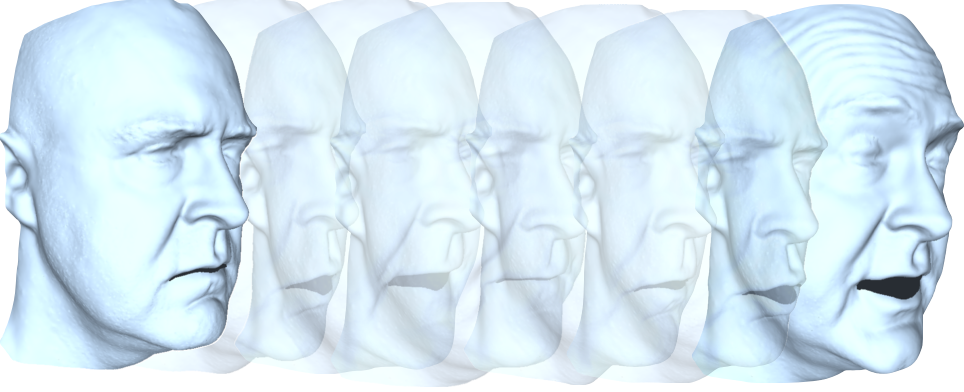
\includegraphics[height=1.5in]{./img/face-seq.png}
\end{figure}
\end{frame}

\begin{frame}{Glance}
\begin{figure}[!htb]
\centering
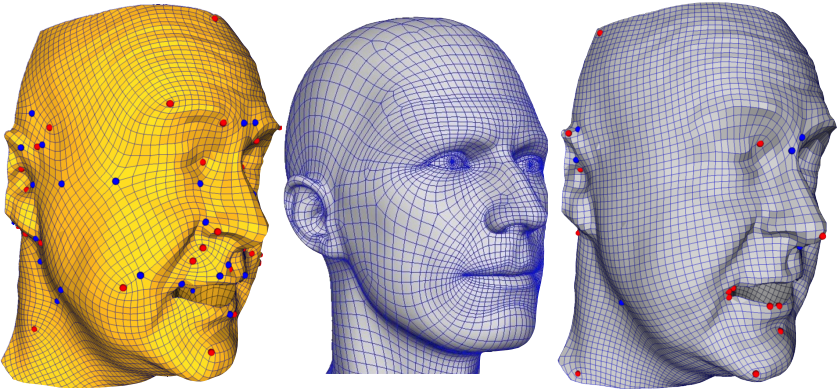
\includegraphics[height=1.5in]{./img/face-quad.png}
\caption{Left: result of this paper. Middle: designed by artist. Right: result of MIQ.}
\end{figure}
\end{frame}

\section{Key Idea}
\begin{frame}{Key Idea}
\begin{block}{Key}
They require vector field to fit deformation gradient.\\
In a sense that: $\min E(F)=\|F-\nabla f\|$
\end{block}
For the other parts of quad generation, they use the same frame work as MIQ.
\end{frame}

\section{Algorithm}
\begin{frame}{Algorithm}
\begin{block}{Keey 4-RoSy orthogonal}
\begin{eqnarray}
J&=&U\Sigma V^T=\underbrace{UV^T}_{R}\cdot \underbrace{V\Sigma V^T}_{S}\\
JV&=&U\Sigma
\end{eqnarray}
\end{block}
Colums of $U,V$ and principal directions of $J,S$ respectively. They are \textcolor{red}{orthogonal}.
\end{frame}

\begin{frame}{Algorithm}
\begin{block}{Fit all poses}
For a sequence Meshes: $\{M_0,...,M_n\}$, each $J_{0,k}$ defines an ideal direction of $M_i$ in $M_0$.
The best fit direction is:
\begin{eqnarray}
\bar{\theta}_t=\frac{1}{4}\Phi(\frac{\sum_i s^i_t \Psi(4\theta^i_t)}{\sum_i s^i_t})
\end{eqnarray}
where $\Psi(\theta):=(\cos(\theta),\sin(\theta))$, $\Phi(\theta):=atan2(y,x)$ , $s_t^i=\frac{min(s_1,s_2)}{\max(s_1,s_2)}-1$.
\end{block}
\end{frame}

\begin{frame}{Direction Field Generation}
\begin{block}{Smoothness Measurement}
\begin{eqnarray}
E=(1-\alpha)\sum_{e_{i,j}\in \xi}(\theta_i+k_{e_{i,j}}+\frac{\pi}{2}p_{e_{i,j}}-\theta_j)^2+\alpha \sum_{t\in \mathcal{F}} s_t(\theta_t-\bar{\theta}_t)
\end{eqnarray}
where $s_t=\frac{\sum_i s^i_t*s^i_t}{\sum_i s^i_t}$. This design of $s_t$ is used to hightlight large deformation of only a few frames in a long sequence.
\end{block}
\end{frame}

\section{Results}
\begin{frame}{Results}
\begin{figure}[!htb]
\centering
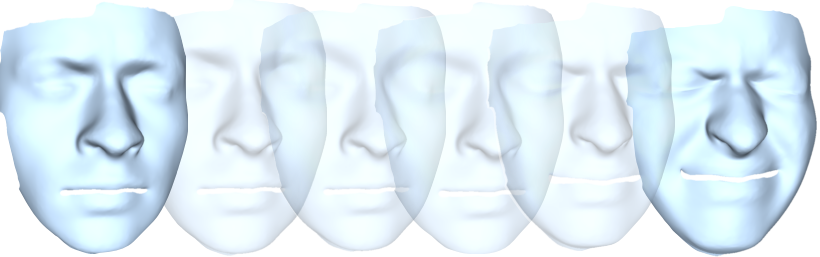
\includegraphics[height=1.2in]{./img/face-seq-2.png}\\
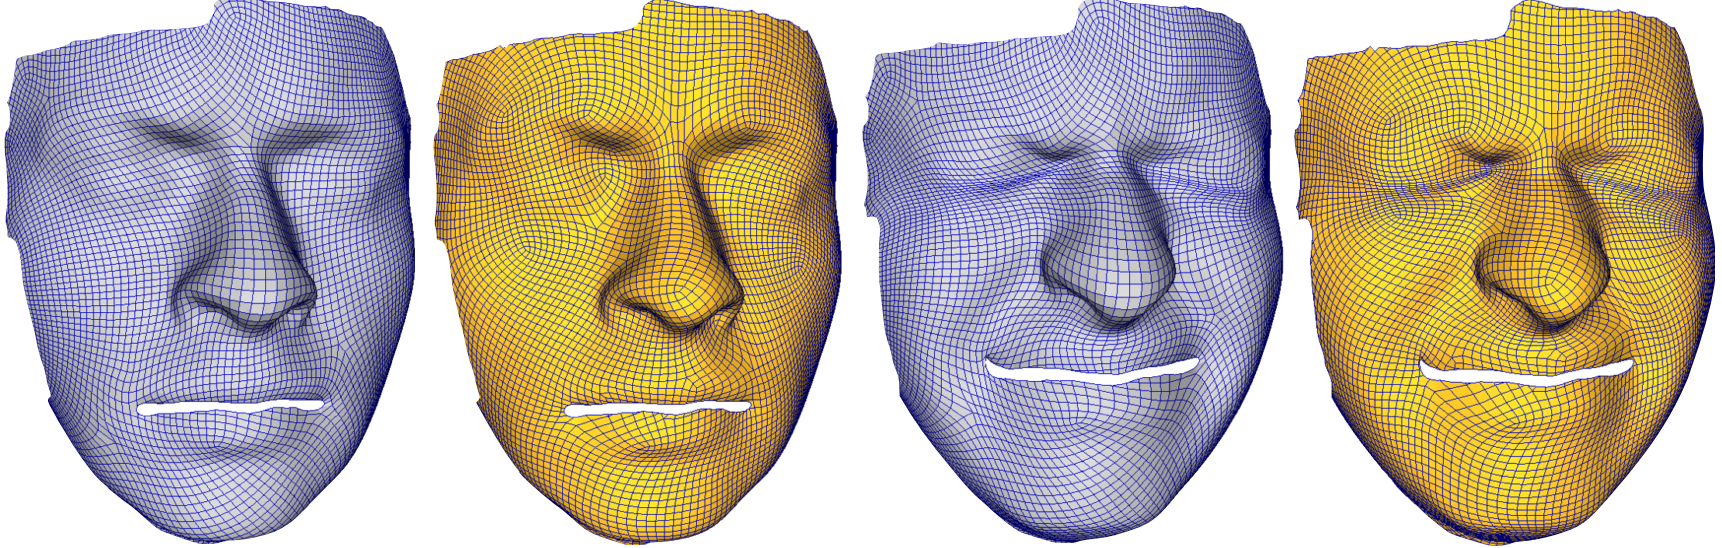
\includegraphics[height=1.2in]{./img/face-quad-2.png}
\caption{Yellow: result of this work. Grey: result of MIQ.}
\end{figure}
\end{frame}

\begin{frame}{Results}
\begin{figure}[!htb]
\centering
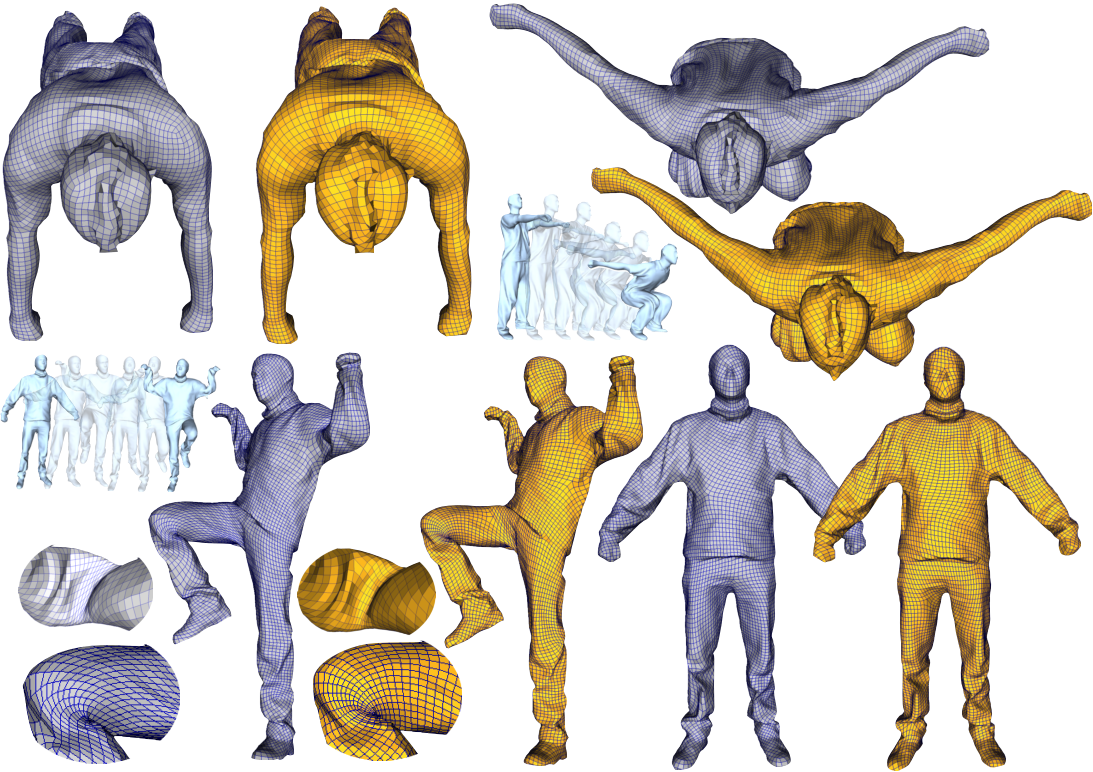
\includegraphics[height=2.5in]{./img/human-seq.png}
\caption{Yellow: result of this work. Grey: result of MIQ.}
\end{figure}
\end{frame}

\section{Conclusion}
\begin{frame}{Conclusion}
\begin{block}{What I like:}
\begin{itemize}
\item A new view of vector field generation, not only geometry property but also deformation requirement.
\end{itemize}
\end{block}

\begin{block}{What I dislike:}
\begin{itemize}
\item Weight of large deformation in eqn 4 is too rough. \\ Here, a problem should be think carefully: should we design a quad according to the largest deformed shape or the averaged shape?
\end{itemize}
\end{block}
\end{frame}

\begin{frame}{}
\hspace{1.5in}\huge{Thank you!}
\end{frame}
\end{document}
